\chapter{The Language of Spices}
\label{ch:language}

% \setlength\intextsep{0pt}

% Empirical Chapters
% Discuss and present your findings in a factual way.
% What are the results of your investigations?
% How do the findings relate to previous studies?
% Was there anything surprising or that didn’t work out as planned?
% Are there any themes or categories that emerge from the data?

\lettrine[lines=\iniciale]{\textcolor{\accentcolor}{N}}{ow} that the detailed explanation of the diffusion of spices is complete, let us examine spice names. Throughout this chapter, I will look at the terminology comparatively, using three sets of names representing spice nomenclature in English, Arabic, and Chinese. This chapter constitutes the results and findings of the analysis on the terms of the spice domain, from linguistic-cognitive perspectives. 

I will start with an overview of the data and the results in numbers, and then I will thematically introduce certain aspects of the terminology, guiding the reader from a general questions of analyzability and structure, towards more nuanced probes that will shed light on the composition, rationale, and motivations behind spice names. The aim of this section is to have an understanding of how spice names are formed, what are the components of typical spice names, and why languages use these elements. At the end of this chapter, a close look into the names of one specific spice will show how can we apply the findings. 

\section{Overview: Spice Names in Numbers}
% Figures and Statistics

\begin{wrapfigure}{R}{0.33\textwidth}
  \vspace{-\baselineskip}
  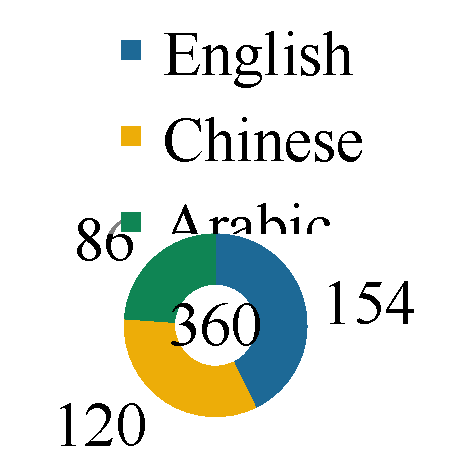
\includegraphics[width=0.33\textwidth]{imgs/plots/languages_pie.pdf}
  \caption{The distribution of spice names across the three languages.}
  \label{fig:languages_pie}
\end{wrapfigure}

As a result of the data collection set forth in \cref{ch:data}, the spice name dataset now contains 360 spice names. Of these, 154 are in English, 86 are in Arabic, and 120 are in Chinese; \cref{fig:languages_pie} shows this distribution.
The total number is the result of the lengthy process of carefully compiling the nomenclature for the set of spices as defined at the beginning of the thesis, which consists of 24 different spices. The data collection methods were detailed in \cref{sec:data_collection}. Combing through dictionaries and the literature, it quickly became clear that the accumulation of spice names---and therefore this project is essentially endless---there is no feasible way to compile the infinite aromatic plant products of the world, and certainly not their many names. This can spark both stress and joy; on the one hand I am relieved that I chose only two dozen relatively well-known spices and not more, while on the other I am excited to see that there is room to grow: there are more aromatics to include, more names to examine, and more things to learn.
 
On average, a spice in my dataset has 14 names, where the max is 44 (chile), and the min is 4 (fenugreek and mace). \Cref{fig:ids_top_and_bottom_ann} shows the top ten and the bottom ten spices that have the most and least number of names, including all three languages. The legitimacy of this figure might raise some eyebrows, but in fact it is a very good indicator of which spices are more complicated in their nomenclature overall, and therefore which are the most \textit{problematic} to untangle. As we can see, spice plants that boast with many names include the chili pepper, Sichuan pepper, cassia and false cardamoms, which represent spices that are rich in variety. On the other hand there is also allspice, which has no variety at all but a confusing and unclear set of names across the three languages. These are---not incidentally---the very items that I have dedicated substantially more pages to than some of their peer spices, due to issues about their identity or the complexity and richness of their nomenclature. This seems to go hand in hand with matters of biodiversity: chile has countless varieties that have spread to faraway corners of the earth, and now it is a hobby in its own right to cultivate, breed, and crossbreed hot chile cultivars. As we saw, Sichuan pepper species are used across vast regions in East Asia (mainly in China), and it can cause headache to pin them down exactly, their ``boundaries'' and varieties are not that well defined---especially to those outside East Asia---and it does need some explanation to untangle and isolate the various sources of cassia types as well.

\begin{figure}[!ht]
	\centering
	\subfloat[]{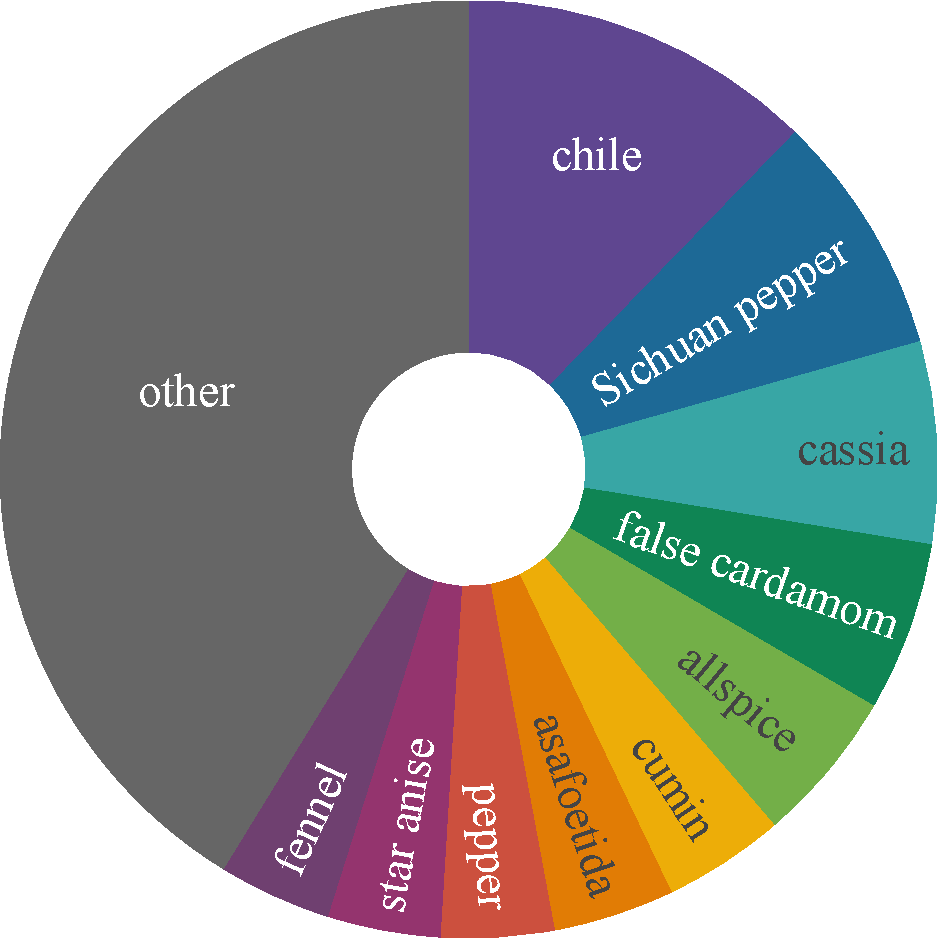
\includegraphics[width=0.5\linewidth]{imgs/plots/ids_top_pie_ann.pdf}}
	\hfill
	\subfloat[]{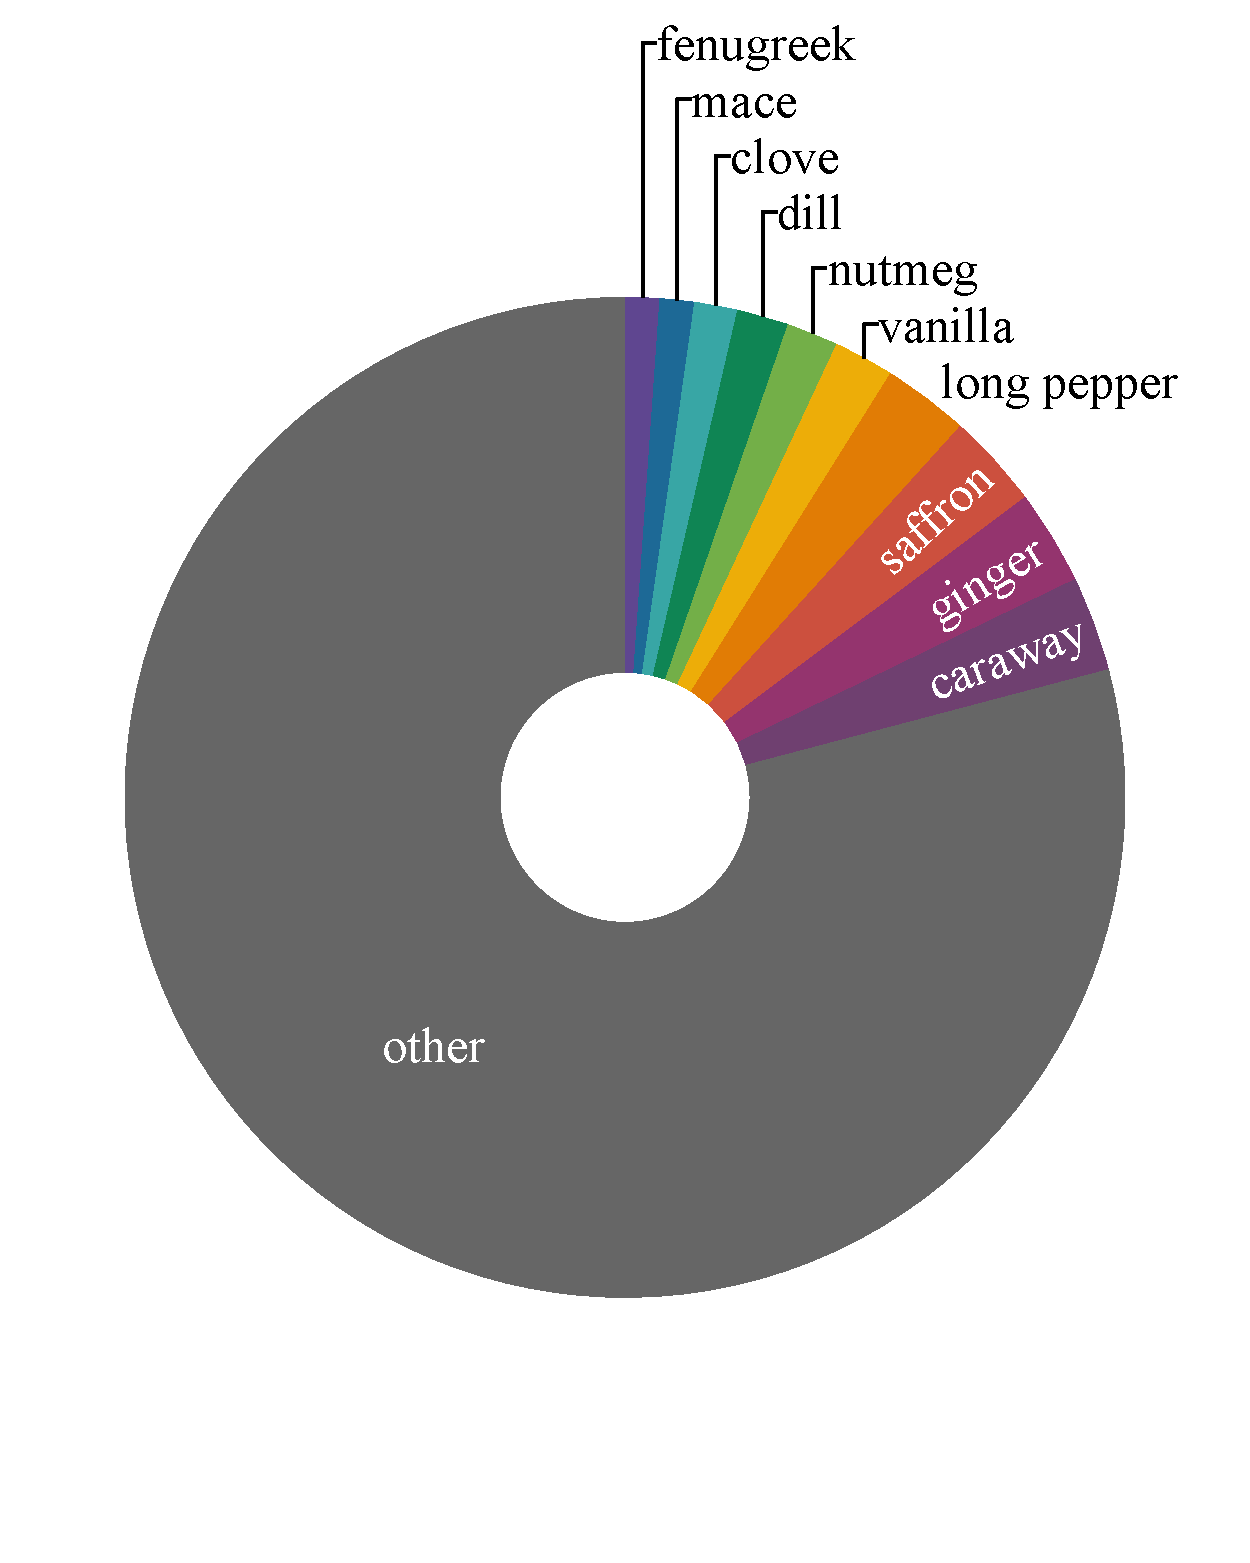
\includegraphics[width=0.5\linewidth]{imgs/plots/ids_bottom_pie_ann.pdf}}
	\caption[Top and bottom spices by number of names.]{Top 10 spices with the most number of names (a), and bottom 10 spices with the least number of names (b).}
	\label{fig:ids_top_and_bottom_ann}
\end{figure}

\begin{figure}[!ht]
	\centering
	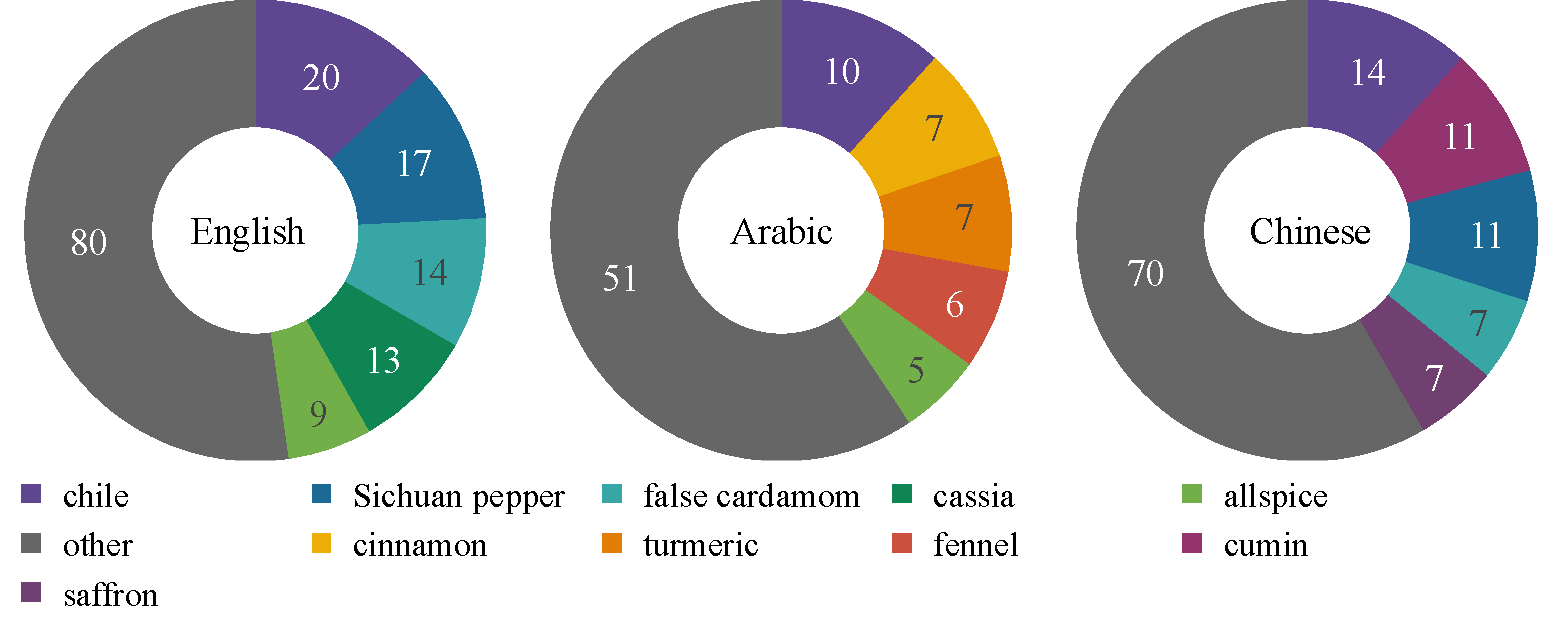
\includegraphics[width=\linewidth]{imgs/plots/ids_tripie.pdf}
	\caption[Top spices by number of names, broken down by language.]{Top 5 spices with the most number of names, by language.}
	\label{fig:ids_tripie}
\end{figure}

On the other hand, spices with the lowest number of names are presumably the most straightforward items, take for example cloves, or vanilla. But what makes a spice ``straightforward'', or in other words, simple? In my opinion, it is their uniqueness and recognizability. Indeed, if we reflect on our investigation on vanilla in the last section of the data chapter, we have already established that it is a rather special item: there is no other spice that is made from the fruits of an orchid, no other spice that is obtained from crystals of long dark brown beans, and no other spice that is sold in liquid form---it is unique. Or, if we think of cloves, they are unmistakable in their shape and in many language they are known by their shape. These two items are also very well circumscribed in terms of their geographic origins. Although now cultivated in multiple tropical regions, vanilla is known to be from the jungles of Central America and Brazil, there is no doubt about its origins. The native habitat of cloves is even more narrow, as it is only indigenous only to North Maluku and the ``spice islands'' of Makian, Ternate, and Tidore. We see nutmeg and mace as well among the bottom five items with the least amount of names, and we should notice that nutmeg and its mace are also from this region, they were exclusively found on the Banda islands of Maluku, and nowhere else until the second half of the \nth{18} century. Now, it makes a bit more sense to look at these same charts deconstructed by language, this can be seen on \cref{fig:ids_tripie}. The most conspicuous feature of these pie charts is that chili has the most names, across every language.



\section{The Analysis of Spice Nomenclature}
\label{sec:analysis}

This section will now present the analysis on spice names trying to answer the main question: How do people name spices, and specifically, new spices that they came into contact with? Immediately, we can think of two ways: languages either borrow, or conceive a name. We saw the borrowed element in the previous chapter, and now we will dive into how the naming process exactly works. What are the  structural requirements and salient features that influence the creation of a name? How languages invent and generate new names for novel materials and substances? In an attempt to give answers to these questions, I took a bottom-up approach and looked at all 360 names of the 24 spices from the data I collected to arrive to some conclusions. 

So what kind of spice names there are? How does a typical spice name looks like? Intuitively, we can identify two core types of names instantaneously along the lines of their structure: \textit{basic, modified}. \textit{Basic} would be a monomorphemic or a derived word that refers to a prototype spice, without any distinguishing word, e.g., \textit{cardamom}. \textit{Modified} could refer to compounds and noun phrases that use a spice name as a headword, but also have a modifier for purposes of identification and disambiguation, e.g., \textit{green cardamom}, \textit{black cardamom}, \textit{true cardamom}, \textit{false cardamom}, \textit{Nepal cardamom}, \textit{Ethiopian cardamom}, \textit{round cardamom}, \textit{lesser cardamom}, \textit{greater cardamom}, \textit{hill cardamom}, etc. We can also discern the wide range of categories of the modifiers referring to color, shape, size, geographic origin, and even positive and negative evaluations of perceived authenticity. A spice term can also have a modifying word to specify the plant part as well, this can be observed most commonly for spices that are known also as plants, or other parts of the plant are used as well, or the same part is used in other form (i.e.,ground or powdered). In English this is usually attached after the headword, similarly to a regular suffix. Examples include: \textit{cumin seed}, \textit{coriander-seed}, \textit{aniseed}, \textit{ginger root}, etc. After consulting intuition, let us consider a more formal analysis.

% Does the nomenclature reflect the contact situation?
% critical factors
% underlying mechanisms

% \subsection{Terminology}
% During the analysis, I will take into account the term's (a) analyzability, their (b) borrowed status, and inspect the ways spice terms are generated using (c) prototype words and distinguishing words.

\subsection{Analyzability and Structure}

Analyzability of words is originally an idea from the \nth{20}-century philological movement and method \textit{Wörter und Sachen} (words and things in German), which had a big influence on linguistics and ethnography. Outlined by Hugo Schuchardt and based on the titular journal \textit{Wörter und Sachen} started by Indo-Europeanist Rudolf Meringer in 1909, it proposed the close study of the etymology of words together with the artifacts/concepts \autocite{ortutay_magyar_1977}. Meringer wrote in 1906: ``Ohne Sachwissenschaft keine Sprachwissenschaft mehr!'' (There is no more linguistics without the study of material culture!). Practically speaking, analyzability meant that the more opaque a name is in terms of morphological analysis, the longer it is assumed to be present in the language. A basic example would be \textit{York} (monomorphemic) vs. \textit{New York} (analyzable), which provides a potential chronology for the concepts the words signify. This approach was incorporated into historical linguistic research and philology, often studied in parallel with findings in archeology \autocite{ortutay_magyar_1977}.

\begin{table}
  \centering
  \begin{tabular}{@{}llrrr@{}}
  \toprule
  \textbf{\#} & \textbf{analyzability} & \textbf{English} & \textbf{Arabic} & \textbf{Chinese} \\ \midrule
  0           & analyzable             & 111              & 50              & 99              \\
  1           & unanalyzable           & 39               & 32              & 20               \\
  2           & semi-analyzable        & 3                & 4               & 1                \\ \bottomrule
  \end{tabular}
  \caption{Analyzability of words in the spice name dataset.}
  \label{table:analyzability}
  \end{table}

\textcite[12]{haspelmath_loanwords_2009} also used the term ``analyzability'' in the creation of their loanword database (\gls{WOLD}) as a first step to assess a word's loanword status, although in a purely linguistic way. I have applied a simplified version of this annotation, and indicated if a word was (1) unanalyzable, (2) semi-analyzable, (3) or analyzable. Items are semi-analyzable if the situation is morphosyntactically complex. For example in case of ``cranberry words'' such as \textit{fenugreek}, where an English speaker could decipher the element \textit{Greek}, but would be left in the dark with \textit{fenu-}, or the Arabicized loanwords from Persian, \textit{dārṣīnī} `cinnamon' or \textit{dārfilfil} `long pepper', where both \textit{ṣīnī} `Chinese' and \textit{filfil} `pepper' would be understood, but Arabic speakers would not know what to do with \textit{dār} (which coincidentally means `house' in Arabic, but it is from Persian `wood'). A Chinese example could be \textit{huluba} `fenugreek', where \textit{hu} `barbarian' is the same character that is found in \textit{hujiao} `black pepper', pointing to its foreign origins, but the whole word itself would be difficult to decode since it is in part a phono-semantic matching or Arabic \textit{ḥulba} `fenugreek'. Sometimes the Chinese term uses the first character 葫, which is a phono-semantic compound of \textit{hu} `barbarian' (after its sound value) and \textit{cao} `herb' for its meaning, making the loanword origin more obvious. 

Analyzability of words greatly interlinks with their structure, which can be simple or monomorphemic (e.g.,\textit{hing}), compound (e.g., \textit{stinking gum}), or phrasal (e.g., \textit{devil's dung}). \textit{Asafoetida} would be considered a compound to those only who are familiar with either Latin, or the history and meaning of this word. Even if we are, \textit{asa} is a cranberry morpheme, and \textit{foetida} `fetida' might not be immediately obvious, so it is a semi-analyzable compound. 

Importantly, compounds that are coined within a language are not considered loanwords, even if they contain borrowed elements. Thus, while \textit{chili} is considered a loanword, \textit{chili pepper} is not. Of course, there are always ambiguous cases: is \textit{black pepper} a loanword? It depends on if it is a learned loan/semantic translation from Latin \textit{piper nigrum}, or a genuine English invention; and for this we have to dig deep into the history of words. To sum up, we could say that if a word is morphosyntactically complex, ``it was almost certain that it was created by speakers of the language rather than borrowed from some other language'' \autocite[12]{haspelmath_loanwords_2009}. 

Words that are analyzable are most often compound in their structure, but there are a few derived names as well. As English is an isolating language, it is less comon to find derived words. Derived terms do occur in Arabic, where a handful of spice names come from verbal roots originally referring to the method of acquisition, such as \textit{qirfa} `cinnamon' from \textit{qarafa} `to peel, derind', or \textit{salīkha} `cassia' from \textit{salakha} `to pull off, strip off; skin, flay'. Other methods of word formation for generating spice names in Arabic include the diminutive pattern, cf. the form \textit{fulayfila} from \textit{fulful} `pepper', equivalent to `capsicum'. Or, the pattern to form an active participle in the feminine as it has been proposed in case of \textit{fāghira} `Sichuan pepper' from \textit{faghara} `to open', alluding to the half open, mouth-like pericarps of \taxon{Zanthozylum} species. There a few examples of phrasal names as well, such as the abovementioned \textit{devil's dung}, but most often these tend to be titles of praise rather than  actual names, for example \textit{king of spices} `black pepper', \textit{queen of spices} `cardamom', \textit{red gold} `saffron', etc. \Cref{table:analyzability} and \cref{fig:analyzability_tripie} show the trilingual distribution on the analyzability of words. Closely related to analyzability, is the question if a term is borrowed or not, which I have already covered in the previous chapter on the diffusion of spice words.

  \begin{figure}[ht!]
    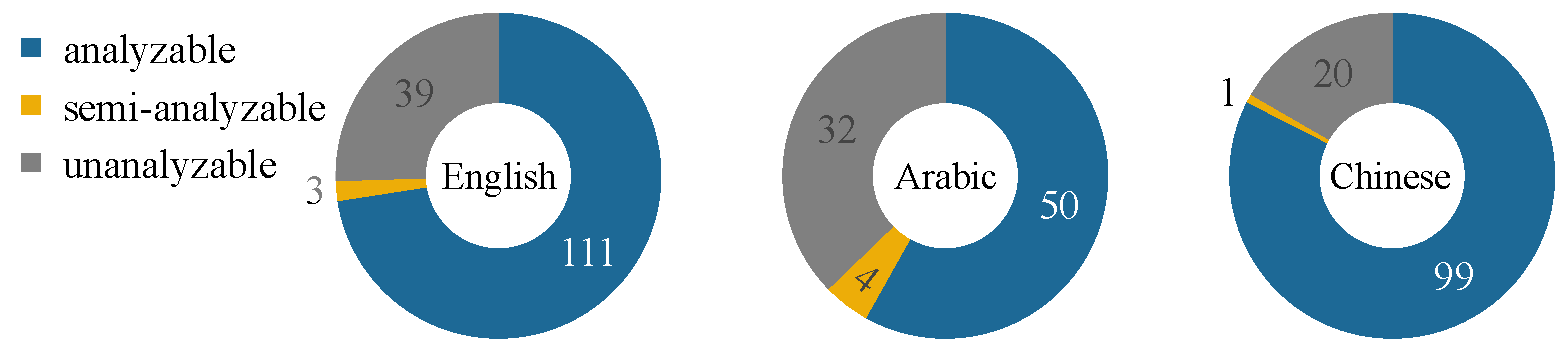
\includegraphics[width=\linewidth]{imgs/plots/analyzability_tripie.pdf}
    \caption{The ratios of the analyzable words in the spice name dataset.}
    \label{fig:analyzability_tripie}
  \end{figure}



\subsection{Spice Term Anatomy: Prototypes and Distinguishing Words}

I already mentioned that the vast majority of analyzable spice terms are compounds, and so let us look at the anatomy of these compounds. By far, most compounds are made up of two elements, sometimes three, but even more is possible. Based on the principle of analyzability explained above we could rightfully assume that the more elements a compound name has, the more culturally \textit{distant} it is, the more unfamiliar its referent is to the speakers of the language. We saw in \cref{ch:diffusion} that the earliest attested words are indeed \textit{short} and monomorphemic in their form, such as \textit{dill}, \textit{fulful} `pepper' and \textit{gui} `cassia'. And in support of this theory we also saw that recently attested words are likely to be polymorphemic compounds, such as \textit{Sichuan pepper}, \textit{fulful ifranjī} `allspice', and \textit{xilanrougui} `cinnamon'. In short, there is an obvious tendency from spimple towards the complex.

Every compound element has a headword, and one (or more) modifier(s). Take for instance \textit{sweet cumin} referring to `anise', where the headword is \textit{cumin}, and the modifier is \textit{sweet}. The use of \textit{cumin} can be explained by the prototype theory; to the person(s) who coined this term, cumin was an already known, ideal prototype for anise, on account of their similarity in their appearance (indeed, the two kinds of seeds look very similar, and they are related plants from roughly similar geographical origins to an English speaker). And so here, we can determine that the rationale for use of the headword is `prototype similarity' with the basis of physical appearance. In most cases, the motivation behind the creation of spice names is simply identification and disambiguation.\footnote{Another interesting type of motivation is promotion/advertisement, as in the case of \textit{grains of paradise}, where the creation of the name was intended to make the spice more desireable for European buyers. Cf. \textit{xiangcao} `fragrant-grass/herb'} Thus, a distinguishing word is needed to differentiate from the \textit{original} cumin, and this word here is \textit{sweet}. The distinguishing words or modifiers often arise from the most salient quality of the materials when compared to the the prototype item: in this case, the sweetness of anise.

The final thing to point out in this example is that \textit{sweet cumin} is not merely an alternative name of anise, it is an \textit{alias}. Under ``alias'', I am referring to the misleading quality of this name, and I would like to emphasize that the prototype words could be used in two ways: matching or not matching. For example: in the compound \textit{white pepper}, the headword \textit{pepper} is used a matching prototype because the referent of the prototype matches the referant of the whole compound (i.e.,white pepper is really pepper). Hence, white pepper is an alternative name which has the role of narrowing, specifying the subtype of pepper in certain situations.Contrastingly, \textit{Jamaica pepper} is an alias, because in the real world the referent of the prototype and the referant of the compound do not match. In these cases, the protoype is used as a headword on account of its similarity---whether physical, chemical, or other.

This difference in how prototypes fill the role of the headword (matching or not) can have serious real world implications, and it is the one single feature of spice names that can cause the biggest confusion. If I may share a personal anecdote. One of my very close friends is working in the family business of importing and exporting various nuts and oil seeds. When a customer ordered a large shipment of black cumin, her boss---her sister---mistakenly ordered cumin. Now, if my friends sister would have glanced on the report my friend made, she would have noticed immediately that black cumin (also known as nigella, \taxon{Nigella sativa}) and cumin (\taxon{Cuminum cyminum}) are two different spices, from different families. The mistake cost a lot to the company, and a lesson was learned, but we can safely assume that this kind of mixup happens regularly. To be clear, I do not want to ``fix'' the usage of common names in this thesis, I am simply trying to explore and explain why there is confusion between certain materials, so that I can organize and present it in a way that it one day might be useful as a trustworthy checklist or master list of spice names. Right now, I still believe that botanical names are the safest way avoid accidents like this. 

By the way, to make things much worse, there are more than one spices that can be called \textit{black cumin} besides nigella, \taxon{Bunium bulbocastanum} (a.k.a. great pignut), and especially \taxon{Elwendia persica} (black seed, black cumin, black caraway) is often confused with the black seeds of nigella. It is not uncommon for a name to be used for the products of several different aromatic plants, and this is a source of confusion.

% Malagueta pepper (a chili cultivar from Brazil)
% melegueta pepper (Aframomum melegueta)

% https://sunnah.com/bukhari:5687
% Sahih al-Bukhari 5687



\subsubsection{Headwords and Prototypes}

\begin{figure}[ht!]
  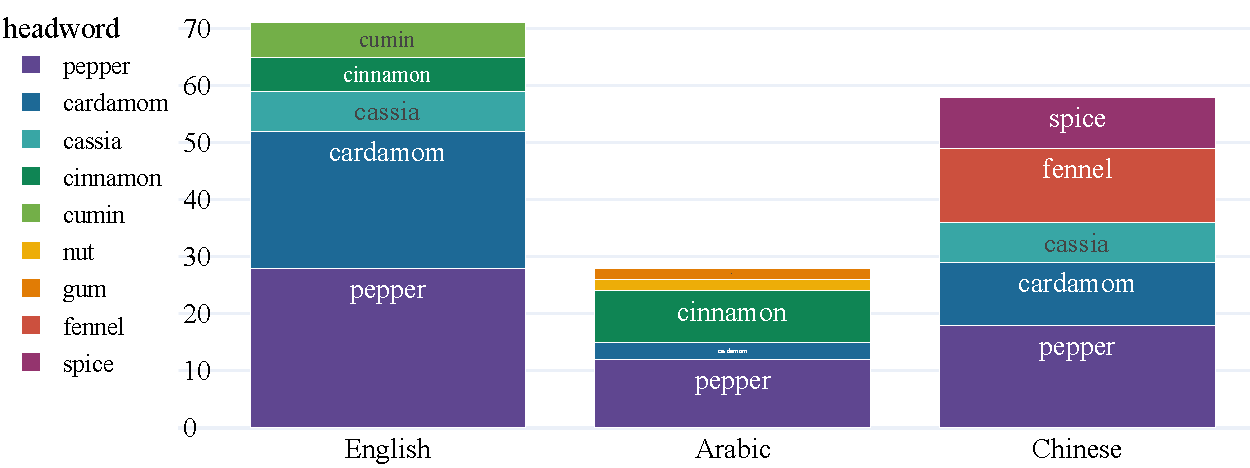
\includegraphics[width=\linewidth]{imgs/plots/headword_bar.pdf}
  \caption{Top 5 headwords appearing in spice names, by language.}
  \label{fig:headword_bar}
\end{figure}

When it comes to frequent headwords, we will most often find spice name prototypes---both matching and not matching the referent of the whole compound---for example, the prototype words for pepper, cardamom, cinnamon, and fennel occur in high numbers. The top most frequent headwords can be seen on \cref{fig:headword_bar}. There are also headwords that do not refer to spices, but rather signify other plant parts and products, such as Arabic \textit{jawz} `nut' (with the pimary sense of `walnut' but by extension any nut) as in \textit{jawz al-ṭīb} [nut-of.fragrance] `nutmeg'. Arguably the most salient feature of the nutmeg is its nut-like appearance, and English also testifies to this. Another example could be the words for gum, referring to the useful part of the ferula plant, asafoetida. Headwords that allude to the function, role, and usage of the substances are also present, consider the \textit{spice} in \textit{allspice}, \textit{bahār} `spice' in \textit{bahār ḥulw}	[sweet-spice] `allspice', or \textit{huixiang} [Muslim-spice] `fennel' or \textit{dingxiang} [nail-spice] `clove'.

\begin{figure}[ht!]
  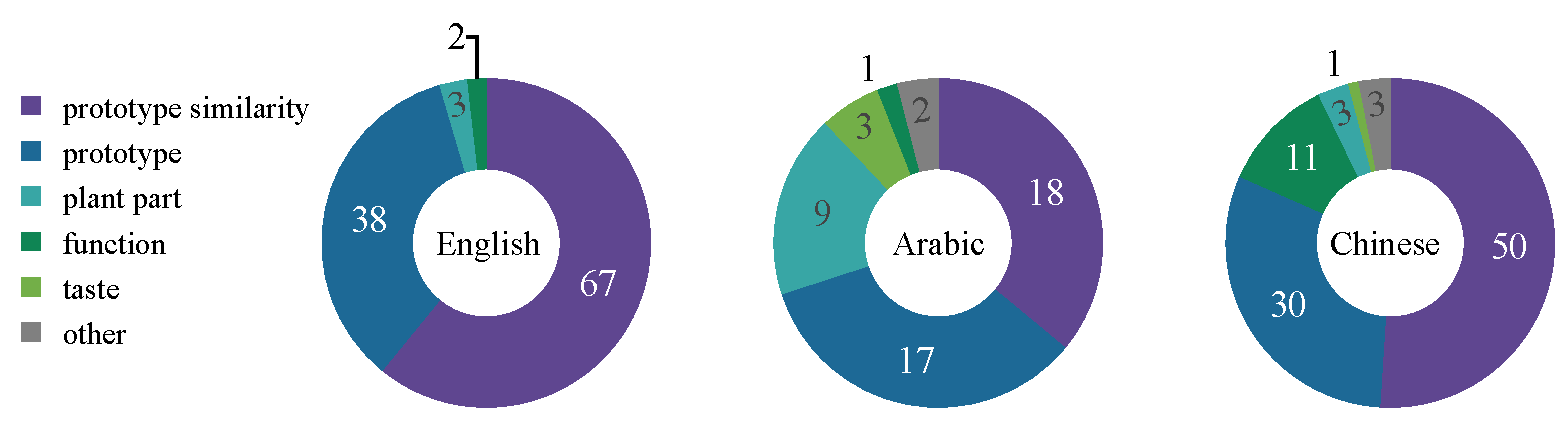
\includegraphics[width=\linewidth]{imgs/plots/headword_type_tripie.pdf}
  \caption{Top 5 headword types in spice names, by language.}
  \label{fig:headword_type_tripie}
\end{figure}

To have an outlook on the full extent of how headwords operate, I have tried to categorize them. According to the usage, most headwords are prototype words used because they are similar to the item that bears he name, followed by cases when the prototypes used matchingly. The rest are a few cases that utilize words of plant parts, function, taste, shape, and color in their headwords as most salient elements.




\subsubsection{Modifiers and Distinguishing Words}

\begin{figure}[ht!]
  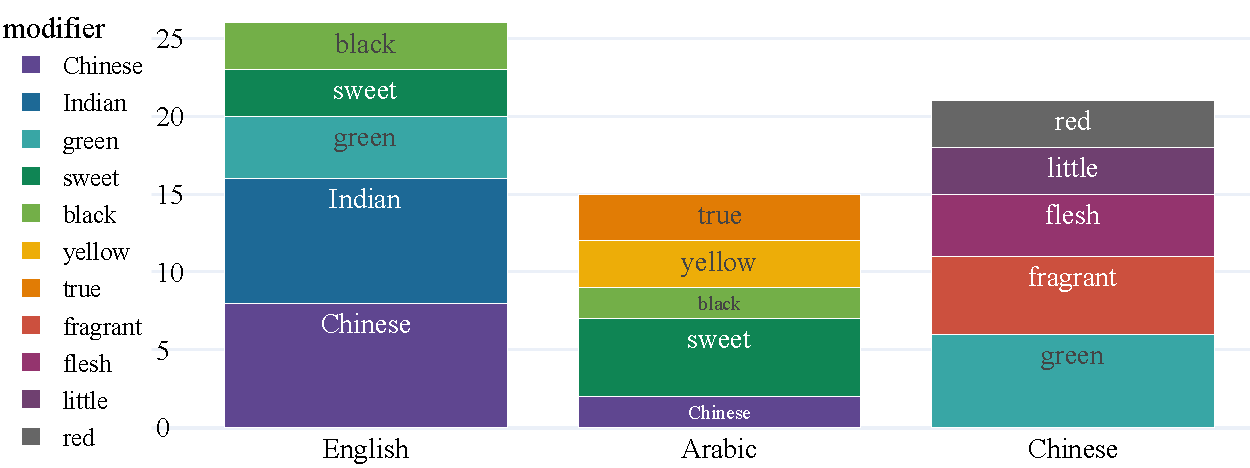
\includegraphics[width=\linewidth]{imgs/plots/modifier_bar.pdf}
  \caption{Top 5 modifiers appearing in spice names, by language.}
  \label{fig:modifier_bar}
\end{figure}

When it comes to modifiers, we can see that the most prominent distinguishing words are adjectives of color, taste, size, shape, but unmistakably, modifiers pointing to geographical origins. Names of countries, regions, cities, perceived or real sources of spices are the most prevalent category here. \Cref{fig:modifier_bar} show the top five modifyers across the three languages. 

% Among the top modifiers in English, we can see \textit{Indian} and \textit{Chinese}, 

\begin{figure}[ht!]
  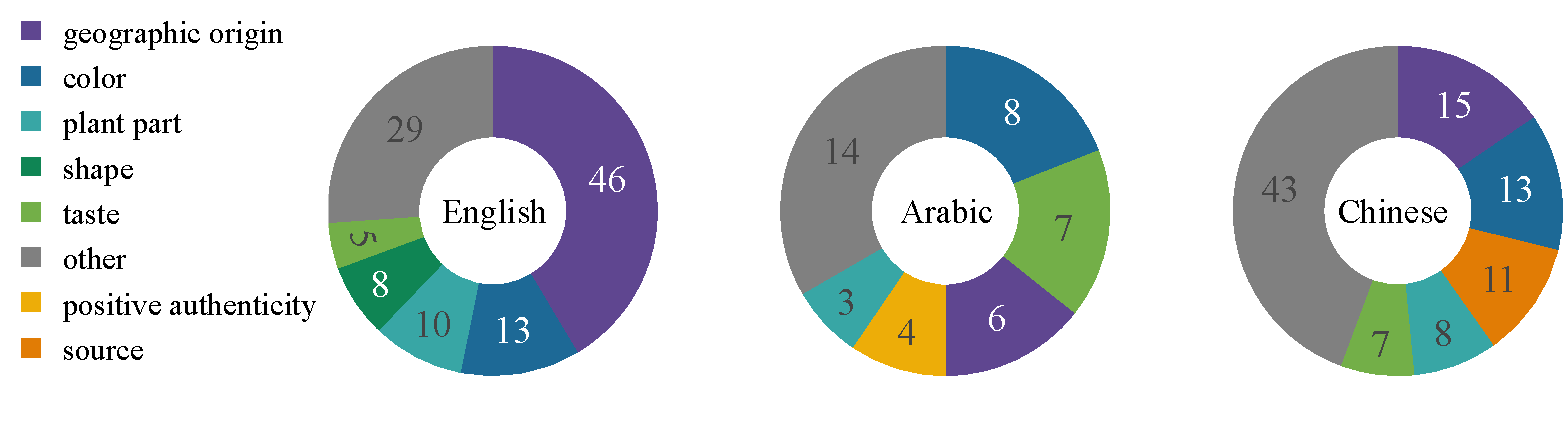
\includegraphics[width=\linewidth]{imgs/plots/modifier_type_tripie.pdf}
  \caption{Top 5 modifier types in spice names, by language.}
  \label{fig:modifier_type_tripie}
\end{figure}

\subsubsection{Sensory Words}

Due to the highly stimulating nature of spices, sensory words often frequent the modifiers. In fact, after distinguishing spices by their geographic origin, the second most common types of modifiers are words of color. What are other salient qualities of perception when it comes to spices? It must taste and smell, right? In my analysis, I have identified and categorized sensory words according to the sensory modalities they operate in and the results can be seen in \cref{fig:sensory_tripie}. It is clear that vision---generally accepted as being part of the ``higher senses'' along with hearing---takes the highest ranks, and the ``lower senses'' follow suit: words from the gustatory, olfactory, tactile, and thermal sensory domains. 

% The term málà is a combination of two Chinese characters: "numbing" (麻) and "spicy (piquant)" (辣), referring to the feeling in the mouth after eating the sauce.

% The numbness is caused by Sichuan pepper, which contains hydroxy-alpha-sanshool

\begin{figure}[ht!]
  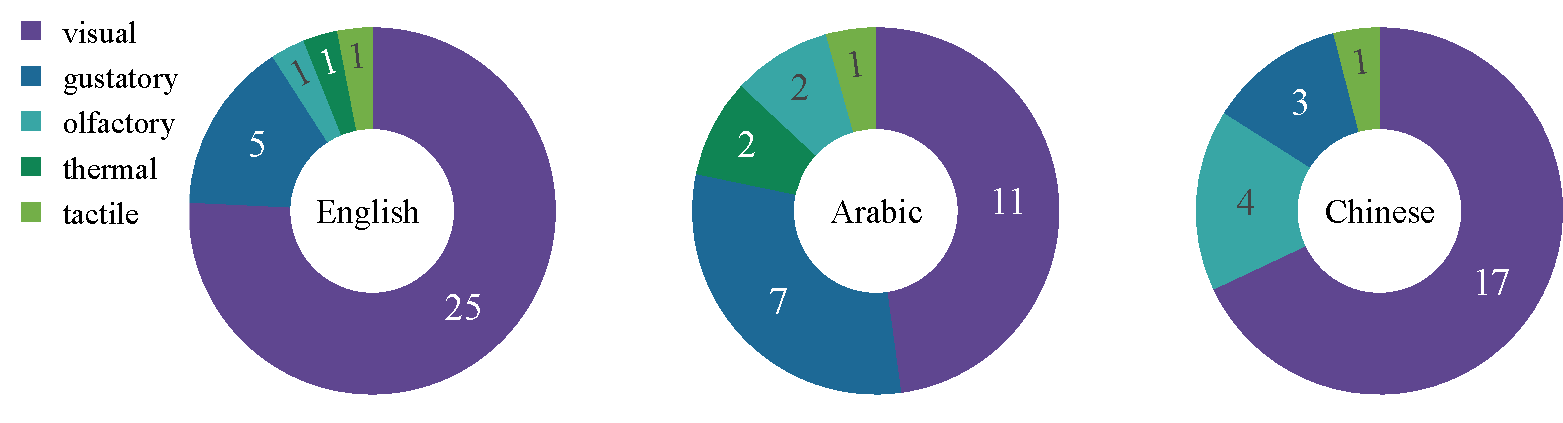
\includegraphics[width=\linewidth]{imgs/plots/sensory_tripie.pdf}
  \caption[Proportion of the sensory modalities in among the modifiers.]{Proportion of the sensory modalities in among the modifier words that belong to a sensory domain.}
  \label{fig:sensory_tripie}
\end{figure}


% Besides adjectival modifiers, there is another usual way to compound spice names, with the use of plant parts.


\subsubsection{Summary}

The final question offers itself: What is the most common blueprint for a spice name? According to the statistics of the dataset, the most common combination is \textit{prototype similarity} + \textit{geographical origin}. Therefore, names such as \textit{Indian cardamom}, \textit{Ceylon cinnamon}, and \textit{Chinese anise} are the most typical examples for naming a spices, where the headwords point to a different item of significant similarity. Therefore, \textit{Jamaica pepper}, the first example we mentioned many pages ago in the introduction, is a fairly regular spice name.





% prototype similarity 	geographic origin 	47
% prototype 	geographic origin 	22
% plant part 	19
% prototype similarity 	color 	16
% prototype 	color 	14
% prototype similarity 	taste 	14

% underlying mechanism

% onomasiology



\section{Spice Name Analysis: The Example of Star Anise}
\label{sec:case_star_anise}

Let us consider the nomenclature of star anise in the three languages. In English, there is the default term \textit{star anise}, which is a native invention, obviously after the fruit's unmistakable appearance. On a rare occasion, we have information on the exact time of star anise's arrival to England, which is dated to 1588.\footcite[star anise]{oed} The same inspiration for the name is found in most European languages, either influenced by 16-\nth{17}-century spice dealer terminology, or devised on their own conviction, looking at its recognizable shape. I used the word ``native'', even though the phrase is obviously mixed from an etymological point of view: \textit{anise} is a loanword ultimately from Greek. However, when faced with this type of phrases, I consider that at the time of the contact situation, \textit{anise} was already part of the English lexicon---as well as \textit{star}---therefore, this phrase was coined within English, and is deemed as a native creation. This practice is consistent with the approach took by the team of \textcite{wold} at \gls{WOLD}. English also has the term \textit{Chinese anise}, which is a phrase consisting of \textit{anise}, again, and \textit{Chinese}, referring to star anise's geographical location and the origin of its procurement for the English. The motivation behind this term could be due to the need to differentiate between Chinese and Japanese star anise, two very similar items. Both phrases utilize the term \textit{anise}, which refers to the small anise seeds of the Mediterranean, used as a spice, and flavoring for liqueurs and confectionary. Why is there a connection to anise? The two plants could not be more different, they are geographically distant, and they are botanically unrelated. The only thing that connects them is their highly similar flavor profile, dominated by the volatile oil anethole; the same nauseating and sweet chemical compound that is found in fennel and licorice. And so, for the Europeans who were familiar with anise and its taste, the novel product reminded them of anise's aroma. Hence, the names are in part inspired by taste/plant chemistry, defining anise as a prototype spice and prototype term. To avoid confusion, (the existence of which will be clear to anyone who tries to do a brief search about anise or star anise), distinguishing words are used for the new material. These modifiers are attached to the headword, and in one case inspired by the spice's shape, on the other hand referring to its geographical origin. The existence of a name of \textit{Chinese star anise} could be explained by the fact that there is a Japanese star anise as well, a similar looking but poisonous fruit and tree, \taxon{Illicium anisatum}, as mentioned above. In short, the two phrases have different ways to identify this spice. English also has an archaic form referring to star anise: \textit{badian} from French, which arrived via a land route through Persian, that might be a phonetic loan from Chinese, but there is no documentary evidence for this.\footcite[badian]{oed}

Arabic \textit{yansūn najmī} [star anise] was devised along similar lines, using a native Arabic word for `star', the prototype word is anise, and the more interesting instances are to be found in neighboring Persian. \textit{Bādyān khatā'ī} or \textit{khatāyī} [star anise] is star anise, while \textit{bādyān rūmī} [Roman anise] is anise.\footcite[Vol. 1, p. 197]{hayyim_new_1934} \textit{Bādyān} alone could also refer to fennel.\footcite[140]{steingass_comprehensive_1892} This shows, that in Persian, the prototype word was \textit{bādyān}. 

As for Chinese, we do not find any loanword among the terms used to refer to star anise, all names are local ``inventions''. The modern ``proper name'' for star anise is \textit{bājiǎohuíxiāng} [eight-horn-hui-spice], where [eight-horn] means `octagonal', and [hui-spice] is fennel, therefore it can be translated as `octagonal fennel', or `eight-horned fennel'. Another name, \textit{dàhuíxiāng} `big-fennel' strengthens the assumption that in Chinese, \textit{huíxiāng} `fennel' is the prototype. Again, the flavor profiles of fennel and anise are basically identical, hence the connection (and confusion). The formal Chinese names of star anise are not attested in historical corpora, and I assume that the vernacular name of \textit{bājiǎo} [eight-horn] was first applied to star anise, and the formal name was modelled later driven by the plant sciences. In modern dialects star anise is also referred to as \textit{huíxiāng} `hui-spice' (historically `fennel') and \textit{dàxiāng} `big-spice'. In modern \gls{TCM}, fennel is referred to as \textit{xiǎohuíxiāng} `little-hui-spice', contrasting the two spices that are confounded due to their taste, using size. In fact, the Chinese \tc{大/小} \textit{dà/xiǎ} `greater/lesser' contrast is not necessarily a marker of size, but a semantic tool to convey unmarked/marked, or proper/imitator.

%%%
% For the use of 大/小  to refer to 

% This is fairly well known but DING Jing's PolyU thesis (and later book published in Springer in 2019(?)) is the most comprehensive semantics of the use of opposites in Mandarin. Not similar 'unmarked' interpretation also show up in English morphosemantics in a different context (e.g.,length, width)...Even though 大/小 is typically translated as greater/lesser, it is somewhat misleading. Trandiationally, 大 is use more often, such as in almost all dynastic names,  大秦/大漢/大唐 . These are simply 秦/漢/唐 without 'lesser'-x in contrast. They are simply indicating an unmarked = 'the proper' meaning. 小登科 little_NameAnnounced is not real 登科 NameAnnounced "success in testing to be imperial official", but 'getting married'.  Modern Mandarin rarely uses this contrastive 大 to undeliner (un)markedness but uses 小, e.g.,小東京 小台北 小巨蛋 小聯合國  they typically to 'something that aspires to be x (and is not a real x). And occasionally both terms are used in contrast, such as 
% 大米 rice 小米 millet; 大年夜 new year's eve 小年夜  the night before new year's eve, 大月氏/小月氏 differentiate the Yuezhi proper (where they have their own kingdom) and 'lesser' (the remaining population that was conquered) 
%%%

To summarize the points I intended to make above: First, I determined if the words and phrases are analyzable (morphologically, syntactically, semantically), then I examined those names further, while also stating why a specific item is unanalyzable. E.g., \textit{badian} as a loanword does not carry any useful information for an English speaker that is not familiar with the word, it cannot be dissected or interpreted alone. Next, I looked at the borrowed status of the names to determine if the word or phrase is borrowed, or devised locally. E.g., the Chinese names are native lexical creations, while English and Arabic use a non-native headword (\textit{anise/yansūn}) and a native distinguishing word (\textit{star/najmī}). Finally, I have looked at the inspirations behind these lexical inventions, and identified the rationale and motivation behind them. For phrases and compound words, we can separate a headword (usually a prototype noun), and a modifier or distinguishing word (usually and adjective). In each case, we can discern the reasons why that prototype word was used, what feature of the prototype item (the referent) is the most salient. The same is true for the distinguishing word(s). For example, \textit{star anise} is named so after (1) similarity in taste + (2) shape; and \textit{Chinese star anise} is named so after (1) similarity in taste + (2) shape + (3) geographic origin. In \cref{table:analysis_star_anise}, you can see a concise overview of the analysis of star anise terminology.

\setlength{\tabcolsep}{3pt}

\begin{table}[!ht]
    \begin{tabularx}{\textwidth}{@{}llLlll@{}} %@{\,+\,}
    \toprule
    \textbf{Term} & \textbf{Gloss} & \textbf{Analyzability} & \textbf{Borrowed} & \textbf{Prototype} & \textbf{Modifier} \\ 
    \midrule
    star anise               &                   & analyzable  & native   & similarity in taste & shape  \\
    badian                   &                   & unanalyzable& borrowed &  &        \\
    Chinese anise            &                   & analyzable  & native   & similarity in taste & origin \\
    Chinese star anise       &                   & analyzable  & native   & similarity in taste & shape + origin \\
    \midrule
    \textit{yansūn najmī}    & star anise        & analyzable  & native   & similarity in taste & shape  \\
    \midrule
    \textit{bājiǎo}          & octagonal         & analyzable  & native   & shape &   \\
    \textit{bājiǎohuíxiāng}  & octagonal-fennel  & analyzable  & native   & similarity in taste & shape  \\ 
    \textit{bóhuíxiāng}      & ship-fennel       & analyzable  & native   & similarity in taste & shape  \\ 
    \textit{dàhuíxiāng}      & big-fennel        & analyzable  & native   & similarity in taste & size*  \\
    \textit{dàliào}          & big-ingredient    & analyzable  & native   & function & size*  \\
    \bottomrule
    \end{tabularx}
\caption{Comparative analysis of the names of star anise in English, Arabic, and Chinese.}
\label{table:analysis_star_anise}
\end{table}
% \multicolumn{1}{c@{\hspace*{\tabcolsep}\makebox[0pt]{+}}}{similarity in taste}

\setlength{\tabcolsep}{6pt}

In this sense, the space names are layered. Intuitively, the more layers a spice name has, the more distant the item was culturally. And on the converse, the less components there is to a term, more familiarity with the substance is presumed (e.g., \textit{anise} vs. \textit{star anise} in English), this reflects back nicely to the idea of the analyzability of words we introduced before. Therefore, spice names' modifiers can be categorized according to what salient feature contributed to the naming the most, and in this specific case, it is star anise's distinct shape. As we will later see, shape is just one of many properties that can distinguish/identify a spice, for others, different properties are salient, including color, taste, smell, and the geographical origin we mentioned. Furthermore, these names reflect on the materials' physical qualities, and the perception and importance of a spice for various sensory modalities in the human experience: vision, gustation, olfaction, etc. 




% Trivially, the more similar some spices are, the more confusing their nomenclature will get. The best example for this are the spices from the umbel family: cumin, caraway, anise, fennel, dill, and so on; little seed-like fruits that grow from the Mediterranean to Central Asia. The fascinating connections are most visible when examining them in multiple languages. % EXAMPLES 

% According to the \gls{WN}, there are four senses to the noun \textit{pepper}. Two refers to \textit{Capsicums}, and two to ``true peppers''. Pepper\#1 in the plant lexical file, with synonyms of common pepper\#1, black pepper\#1, white pepper\#1, Madagascar pepper\#1, and Piper nigrum\#1 is defined as ``climber having dark red berries (peppercorns) when fully ripe; southern India and Sri Lanka; naturalized in northern Burma and Assam''. Its hyponym is pepper\#3, synonym of peppercorn\#1, with the definition ``pungent seasoning from the berry of the common pepper plant of East India; use whole or ground'', now we are in the food lexical file. This latter, has two hyponyms on its own: black pepper\#2 (``pepper that is ground from whole peppercorns with husks on'') and white pepper\#2 (``pepper ground from husked peppercorns'')

% How to accommodate for the confusion in the past, semantic changes kurkum, saffron? They appear twice in both relevant categories! 




% mechanism


% The mechanisms of linguistic acculturation can be deducted from linguistic (and historical) analysis. 
% Is it borrowed or not, and if not, how speakers came up with the name?
% Spices and their spread are related to trade and cultural interaction 
% 	language contact

%     Linguistic acculturation “Response in a language to new items that become known through cultural contact. As the speakers of a language in contact with other cultures encounter new cultural items, they may:”
%     Borrow
%     Loan, calque (loan translate), learned loan…
%     Innovate
%     Compounding, blending, (internal resources)…
%     Shift
%     Narrowing, broadening, displacement…
%     Extend
%     metonymy (e.g.: octogon  bajiao; pentagon  The Pentagon)
%     metaphor
                                                
%                                                         (Campbell & Mixco, 2007)
%                               Borrowing
%                                                         Loanword			anise in English
%                                                         Loan translation		牙买加胡椒 [Jamaica pepper] in Mandarin; ‘allspice’
%                                                         Innovation
%                                                         Compounding		törökbors [Turkish-pepper] in Hungarian; ‘chilli’
%                                                         Folk-etymology		aniseed; safflower (morphological misinterpretation)
%                                                         Shift in meaning		
%                                                         Displacement			pimento in Spanish, replacing pebre ‘pepper’
%                                                         Extension
%                                                         Metonymy			bajiao [octagon] in Chinese; star anise
                                                        
                                                        
                                          


% Star anise is native to South China and Vietnam, fennel is native from Mediterranean to West Asia until the Himalayas. 
% Star anise has been used for around 3000 years (in and around the South, only later in the North), no longer found in the wild.
% The other plants I mentioned are all related to fennel, all are from the Apiaceae, the carrot/celery/parsley family (vt+ coriander 芫荽 and asafoetida 阿魏).
% They all look similar and are used similarly and named after each other in many languages.
% All these plants arrived from the west through Central Asia and the Silk Road.
% This is reflected in some of the names.
% What’s the connection between anise, star anise and fennel?
% Anethole – similar flavor profiles because of the same essential oil

% Is the name native or borrowed?
% The Chinese name is a native Chinese lexical “creation”
% English and Arabic used a non-native headword (anise, a loanword ultimately from Greek<Egyptian?), and a native distinguishing word (star) 


% These names are analyzable. 
% analysability of words is an idea from the philological movement Wörter und Sachen (words and things), which proposed the close study of etymology of words together with the artifacts/concepts.
% The more opaque a name is in terms of morphological analysis, the longer it is assumed to be present in the language.
% E.g.: York (monomorphemic) vs. New York (analysable)  provides a potential chronology
% Incorporated into historical linguistics ( + archeology)




% Just a quick question:
% I couldn't not notice that the character used for fennel and anise 茴 huí is made up of the radical for "grass" and 回 huí which is used for Islam and Muslims in Tang dynasty times. My question is: Could this be a construction that would refer to fennel (or anise) as "Muslim grass", "Muslim herb", since the plant came to China from the West originally (East Mediterranean, Middle East), and most likely through Muslim traders of Central Asia?
% Or this is not how Chinese characters work, and it is just my fantasy running wild and 回 huí is just a sound component...

% Thank you for the answer, I am working on the Tastes of Words article hastily now, I should be done very soon.



% Yes, good observation!  I suspected so too, but could not find direct supporting evidence yet.

% Good indirect evidences, other than your observation, are 
% >that 茴 is not found in Shuowenjiezi, which means that it is a later coinage and most likely borrowing; and in this case, 香 standing for herb in a compound and the first character will typically specify its origin (if borrowed), or plant, or sound
% >the earliest documented usage we can see now of this term is after Tang dynasty (supporting the borrowing hypothesis and consistent with the time of introduction of this herb to China)
% >The only document I found claims that it is derived from 蘾 from SWJZ characters due to phonological similarity. But this is an apparent 'backformation' speculation as 1) the phonology is distinctive enough (huai2 in Mandardin), and 2) it is a kind of watergrass in SWJZ, and definitely no fennel (and of course we do know now that China did not have fennel during SWJZ time)



% \section{What's in a name?}






% \section{Prototype Spices}

% \begin{itemize}
%     \item cardamom
%     \item pepper
% \end{itemize}


% cumin
% anise
% cinnamon
% saffron






%%%%%%%%%%%%%%%%%%%%%%%%%%%%%%%%%%

% \chapter{The Language of Spices}
% \label{ch:language}


% Discussion Chapter
% Discuss and relate your findings to the literature review and theory framework.
% Do so in such a way that a layperson can understand your argument.
% How do the findings relate to the theory and methods discussed previously?
% Why you have reached particular conclusions?
% How do your findings relate to the gaps in the literature you identified earlier?
% What implications do the findings have for the discipline and for existing understanding?
% How do the findings relate to your research questions, aims and objectives?

%------------------------

% This chapter presents an inquiry with classic corpus linguistic methods into spicy words

% This chapter presents the various ways spice terms have established themselves in our daily language, illustrating that they---some more than other---are deeply embedded in the collective human experience. From the earliest of times, since humans started to uses spices as medicine, incense, perfume, and condiments, they left their mark in our vocabulary. This, of course, includes fluctuations varying by region and historical periods, and certain substances enjoyed a higher esteem than others at any given time. 

% My hypothesis is that the more a... 



% \section{Spices in Corpora}

% distribution/frequency

% different spices are more prevalent in different languages/cultures, showing their importance

% mention hindi?

% spoken corpora?

% \subsection{}

% word sketches

% modifiers modified
% what can we learn

% \subsection{Historical Corpora}

% some diachronic comparison?

% \section{Spice Terms and Word Classes}

% use sketch engine to check for adjectives then verbs

% \subsection{Spice Terms as Adjectives}

% spicy

% peppery

% salty?

% \subsubsection{Spices Names as Colors}



% \subsection{Spice Terms in the Verb Paradigm}

% to spice up

% to pepper

% \section{Spices as Metaphors and in Idioms}

% doukou is virgin/maiden age

% 虎辣人 hularen peppery or short-tempered person 395 defrancis

% then check metaphors and idioms

% to have pepper in the nose
% hungarian paprikas hangulat

% different spices in different cultures

% Examples:

% https://en.wiktionary.org/wiki/%E8%B1%86%E8%94%BB


% %------------------------------------------
% \section{\textsc{Spice} in language}

% \subsection{English}

% \subsection{Chinese}

% 辣 ① peppery; hot ② sharp; spicy; biting (of smell/taste) ③ vicious; ruthless 
% defrancis 525



